% !TeX encoding = UTF-8
% !TeX spellcheck = en_US
% !TeX root = main.tex

\chapter{Localization of orbit perturbations}
\label{sec:localisation}

Correcting the orbit is costly and has never a perfect result. Instead of dealing with the effects, the sources of the distortions can be investigated. If none is really obvious (e.g. a non-isolated transformer, the 50~Hz perturbation of the main power), the orbit itself can give some hints.

The place where the orbit brutally changes its angle (as shown in \cref{fig:kick}) is termed \textit{kick}.

\begin{figure}[!h]
	\centering
	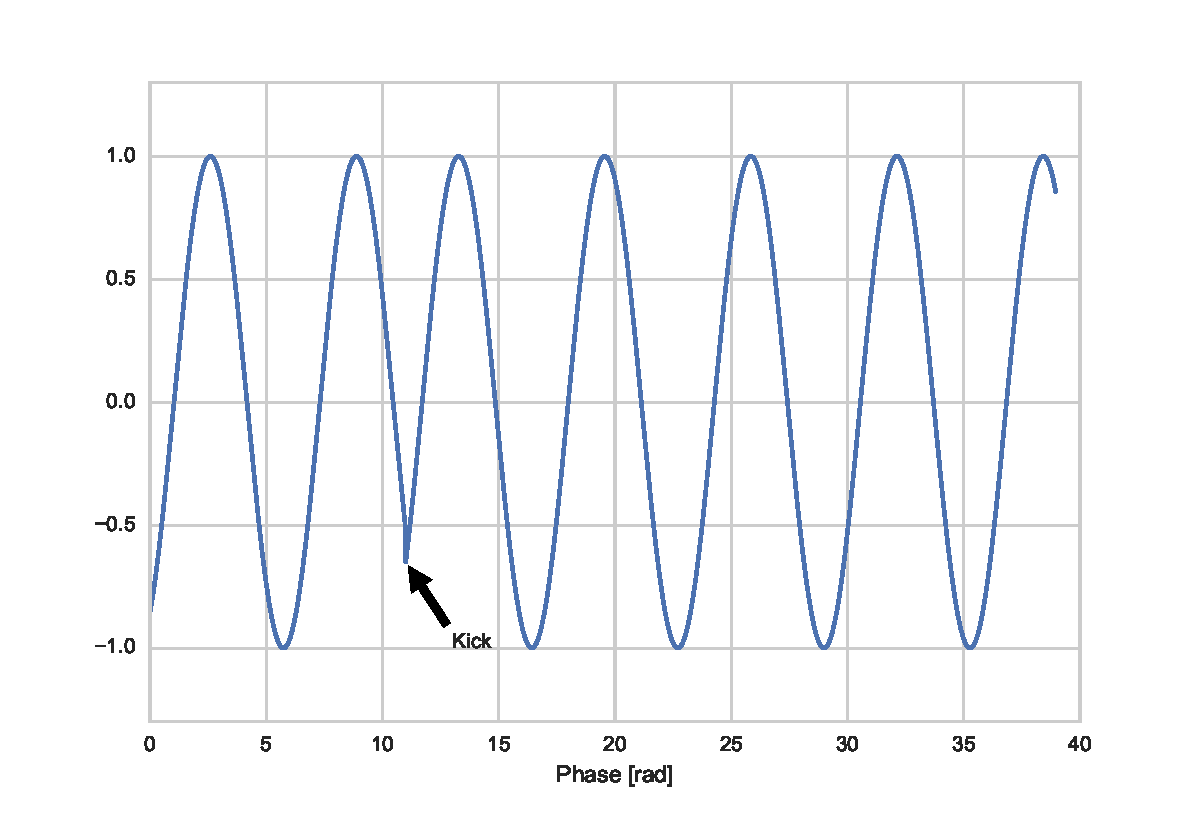
\includegraphics[width=.9\linewidth]{img/kick}
	\caption{\label{fig:kick}Example of kick in the orbit}
\end{figure}

\section{Static perturbation}
\label{sec:loc_static}

\subsection{Theoretical setting of the problem}

Everything is described here with the phase variable 
\begin{equation}
\Psi = \int\limits_{0}^s \frac{d\sigma}{\beta(\sigma)}.
\end{equation}
The spatial variable is only used to have a connection between the result and the actual ring. The explanation will be led with the $x$ variable, but is also valid with the $y$ one.

Let one kick be at $\Psi = \hat{\Psi}$. The orbit is modified and oscillates with a constant period of $2 \pi$. Because there is {\em only one} kick and according to the closed orbit condition, the oscillation after the kick will be stable for one revolution. Furthermore, the orbit must be continuous on all points, thus at the kick position too.

Two revolutions are considered, in order to be sure to find one full revolution without kick. Let $\Psi_\mathrm{ext} \in [0, 4 \pi Q]$ be this new phase (\textit{ext} for extended). The phase $\Psi_0$ where the kick happens is the one so that 
\begin{equation}
\exists (b, c) \in \mathbb{R}^2:
\forall \Psi \in [\Psi_0, \Psi_0 + 2 \pi Q], \quad
x(\Psi) = b \sin(\Psi + c)
\end{equation}

This problem has 3 unknowns which should be determined: $\Psi_0, b, c$. 

\subsection{Practical setting}

Only $m$ BPMs are distributed around the orbit. The previous variable can thus be described in a vectorial form
\begin{align}
\begin{cases}
\vec{\Psi} = [\Psi_0, \Psi_1, ..., \Psi_{m-1}] \\
\vec{x} = [x_0, x_1, ..., x_{m-1}]
\end{cases} \quad \mathrm{and} \quad
\begin{cases}
\vec{\Psi}_\mathrm{ext} = [\vec{\Psi}, \vec{\Psi}+2\pi Q ]\\
\vec{x}_\mathrm{ext} = [\vec{x}, \vec{x}]
\end{cases}
\end{align}

\subsection{Solving the problem}

The problem is solved in two steps: first the sine that fits at best the orbit is determined, and second the position of the kick verifying the closed orbit condition (or continuity condition) is found.

An algorithm is designed to find a sine over a revolution, beginning at each BPM and keep the one that fits at best:
\begin{align}
\forall k \in &[0, m-1], \nonumber \\
&\begin{cases}
\vec{\Psi}^k = [\vec{\Psi}_\mathrm{ext}(k), \vec{\Psi}_\mathrm{ext}(k+1), \cdots,  \vec{\Psi}_\mathrm{ext}(k+m-1)]\\
\vec{x}^k = [\vec{x}_\mathrm{ext}(k), \vec{x}_\mathrm{ext}(k+1), \cdots,  \vec{x}_\mathrm{ext}(k+m-1)]\\
\tilde{\vec{x}} = \mathtt{fit\_sine}(\vec{x}^k, \vec{\Psi}^k)
\end{cases}
\end{align}

It is then defined
\begin{equation}
k_0 = \underset{k \in [0, m-1]}{\textrm{argmin}}\{||\tilde{\vec{x}}-\vec{x}^k||_2\}
\end{equation}

If there where no noise in the signal, and if the precision over the phase $\Psi$ was infinite, then the kick would be exactly at $\Psi_{k_0}$. However in this case, it can only be said that the kick is around $\Psi_{k_0}$, and the closest sine is $\tilde{x}(\Psi) = b \sin(\Psi + c)$.

To find the exact position of the kick, the property of closed orbit is used: the orbit must be continuous also at the kick phase, which means that $\hat{\Psi}$ is the solution of
\begin{align}
b \sin(\Psi + c) &= b\sin(\Psi+c+2 \pi Q),\\
& \mathrm{with}~ \Psi \in [\Psi_{k_0}-A, \Psi_{k_0}+A] , A>0 \nonumber
\end{align}
or, with the numerical approach, 
\begin{equation}
\hat{\Psi} =  \underset{\Psi \in [\Psi_{k_0-A}, \Psi_{k_0+A}]}{\textrm{argmin}}\{|b \sin(\Psi + c) - b\sin(\Psi+c-2 \pi Q)|\}.
\end{equation}

$A$ was defined with the \textit{try-and-see} method and in the specific case of BESSY~II, $A=\frac{\pi}{4}$ suits.

\remark For this last step, we use a \textit{linspace} between $\Psi_{k_0}-A$ and $\Psi_{k_0}+A$ with more than 1000 points.

\subsection{Finding the good sine}
Several methods are possible to find the best matching sine, for example by using:
\begin{itemize}
	\item a pseudo-inversion
	\item a scalar-product with a sine (resp. a cosine)
\end{itemize}

\paragraph{Pseudo-inversion}
The problem can be set as a linear equation problem as follow.
\begin{align}
&\forall k \in [0,m-1], \tilde{x}(\Psi_k) = a_1 \sin(\Psi_k) + a_2 \cos(\Psi_k) + a \nonumber \\
%
\implies &
\begin{pmatrix}
1 & \sin(\Psi_0) & \cos(\Psi_0) \\
1 & \sin(\Psi_1) & \cos(\Psi_1) \\
\vdots & \vdots & \vdots \\
1 & \sin(\Psi_{m-1}) & \cos(\Psi_{m-1}) \\
\end{pmatrix}
\begin{pmatrix}
a \\ a_1 \\ a_2
\end{pmatrix}
=
\begin{pmatrix}
x_0 \\ x_2 \\ \vdots \\ x_{m-1}
\end{pmatrix} \nonumber
\\
%
\implies &
\begin{pmatrix}
a \\ a_1 \\ a_2
\end{pmatrix}
= 
\mathrm{pseudo\_inv}
\begin{pmatrix}
1 & \sin(\Psi_0) & \cos(\Psi_0) \\
1 & \sin(\Psi_1) & \cos(\Psi_1) \\
\vdots & \vdots & \vdots \\
1 & \sin(\Psi_{m-1}) & \cos(\Psi_{m-1}) \\
\end{pmatrix}
\begin{pmatrix}
x_0 \\ x_2 \\ \vdots \\ x_{m-1}
\end{pmatrix}
\end{align}

The pseudo inverse is calculated in \texttt{Matlab} with 
\begin{verbatim}
        a = M\x
\end{verbatim}
and in \texttt{Python} with the least-squares method
\begin{verbatim}
        a = numpy.linalg.lstsq(M, x).
\end{verbatim}

\paragraph{Scalar product with a sine (resp. cosine)}
Since the orbit is expected to be written as
\begin{equation*}
x(\Psi) = a+ a_1 \sin(\Psi) + a_2 \cos(\Psi)
\end{equation*}
it can also be described as
\begin{equation}
x(\Psi) = \scal{x}{1} + \scal{x}{\sin} \sin(\Psi) + \scal{x}{\cos} \cos(\Psi)
\end{equation}
with $\scal{f}{g}$ being the scalar product for real functions: $\int_T f(t)g(u)dt$.

In the numerical case, the scalar product is approximated by its vectorial counterpart by
\begin{align*}
\scal{\vec{f}}{\vec{g}}: \quad
 &\mathcal{R}^n \times \mathcal{R}^n \longrightarrow \mathcal{R} \\
 & (\vec{f},\vec{g}) \quad\longmapsto \quad \frac{1}{n}\sum\limits_{k=0}^{n-1} f_i g_i
\end{align*}

\paragraph{Coefficient format}
By defining $b = \sqrt{a_1^2+a_2^2}$ and $c = \mathrm{atan2}(a_2, a_1)$ the previous formulas can be written
\begin{equation*}
\tilde{x}(\Psi) = a + a_1 \sin(\Psi) + a_2 \cos(\Psi) = a + b \sin(\Psi + c).
\end{equation*} 

\section{Harmonic perturbations}
In this section, the perturbation is harmonic with a given frequency $f$. The training data is the time signal of all BPMs.

As the perturbation has a known frequency, its complex amplitude can be extracted from the signal of each BPM with a Fourier transform:

\begin{equation}
\forall i \in [1, \mathrm{BPM\_nb}], \qquad 
\begin{cases}
\vec{X}_i = \mathrm{FFT}(\vec{x}_i) \\
c_i = \vec{X}_i(f)
\end{cases}
\end{equation}

\subsection{Case of a unique perturbation source}

If the perturbation is unique, then all complex amplitude exactly describe the same sine of frequency $f$ and phase $\alpha_0$. The complex vector $\vec{c}$ can thus be fully described with $\vec{\hat{c}}$, which is real.

\begin{align}
&\alpha_0 = \underset{\alpha \in [0, 2\pi]}{\textrm{argmin}}\{\mathcal{R}e (\vec{c} \cdot e^{-j\alpha}) \} \label{eq:harm_perturb_opt}\\
&\vec{\hat{c}} = \mathcal{I}m (\vec{c} \cdot e^{-j\alpha_0})
\end{align}

The new signal $\vec{\hat{c}}$ can be used as an orbit signal: each BPM have one orbit amplitude. The kick can be extracted from it with the previous method described in \cref{sec:loc_static}.

\remark To achieve the phase optimization given in \cref{eq:harm_perturb_opt}, the Karhunen–Loève transform (or principal component analysis) can be used~\cite{book:wang_2012}. A description of the algorithm is given in \cref{apx:KLT}. If the results are exactly the same, this allows the problem to be solved within a broader theoretical setting. The goal is not anymore to see the cosine part vanish but to deal with the perturbation space in which the distortion is the largest. In theory, dealing with each principal component would allow to find the position of each perturbation source.

\subsection{Case of several perturbation sources}
If there are several perturbation sources, a $\alpha_0$ that let the cosine part vanish cannot be found. 


\section{Implementation}
\begin{python}[caption=Get the kick]
	import matplotlib.plt as plt
	import search_kick.core as skcore
	
	# Dataset
	orbit = ..
	phase = ..
	tune = ..
	
	# Get the kick and rebuild the ideal sine
	kick_phase, sin_coef = skcore.get_kick(orbit, phase, tune)
	sine, phase_th = skcore.build_sine(kick_phase, tune, sin_coef)
	
	# Plot the results
	plt.plot(phase, orbit, '-b')
	plt.plot(phase_th, sine, '-g')
	plt.axvline(kick, -2, 2)	
\end{python}


\section{Examples}

